% !TeX spellcheck = en_US
\chapter{System description}
The project is a collection of three individually developed systems, who as a whole makes it possible to test and control the AU2.

\section{AU2}
The MCU(Motor control unit) can be seen in figure \vref{fig:SD_MCS} without the PSoC.

\begin{figure}[H]
	\centering
	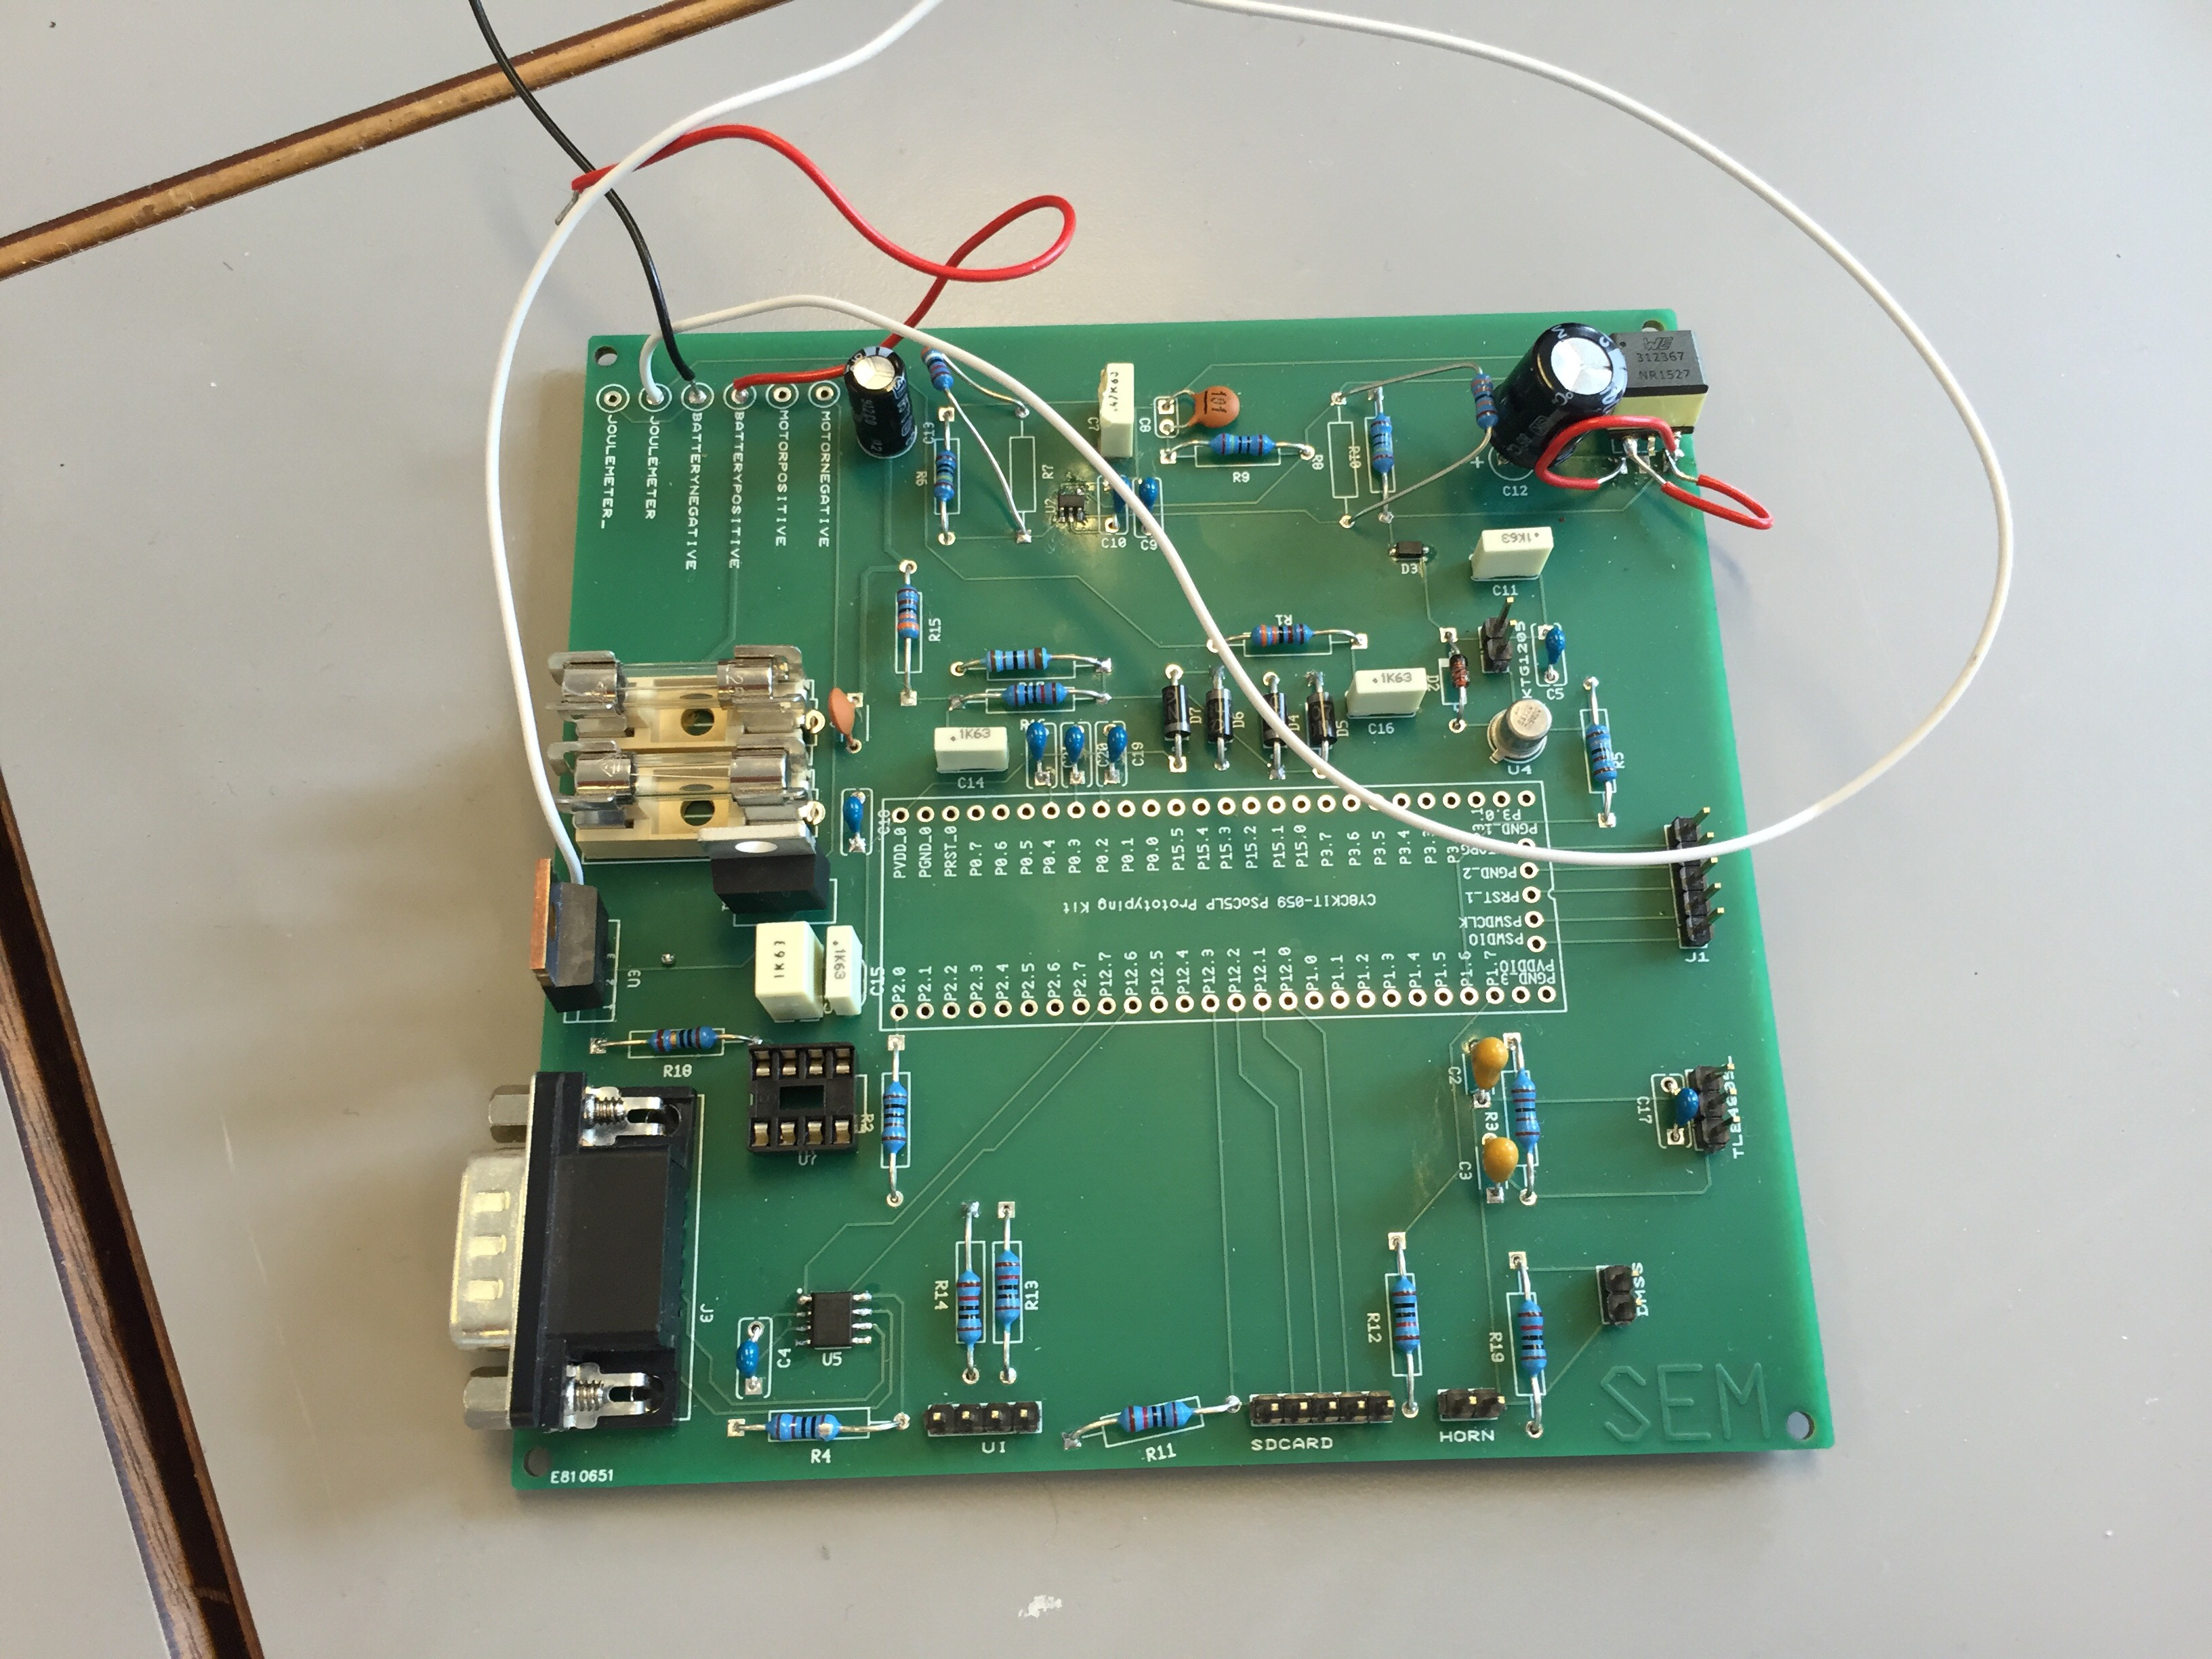
\includegraphics[width=0.6\linewidth]{SubPages/Images/SD_MCS}
	\caption{Motor control system}
	\label{fig:SD_MCS}
\end{figure}

The BMS(Battery manage system) can be seen in figure \vref{fig:SD_BMS}, with the batteries visible in the top.

\begin{figure}[H]
	\centering
	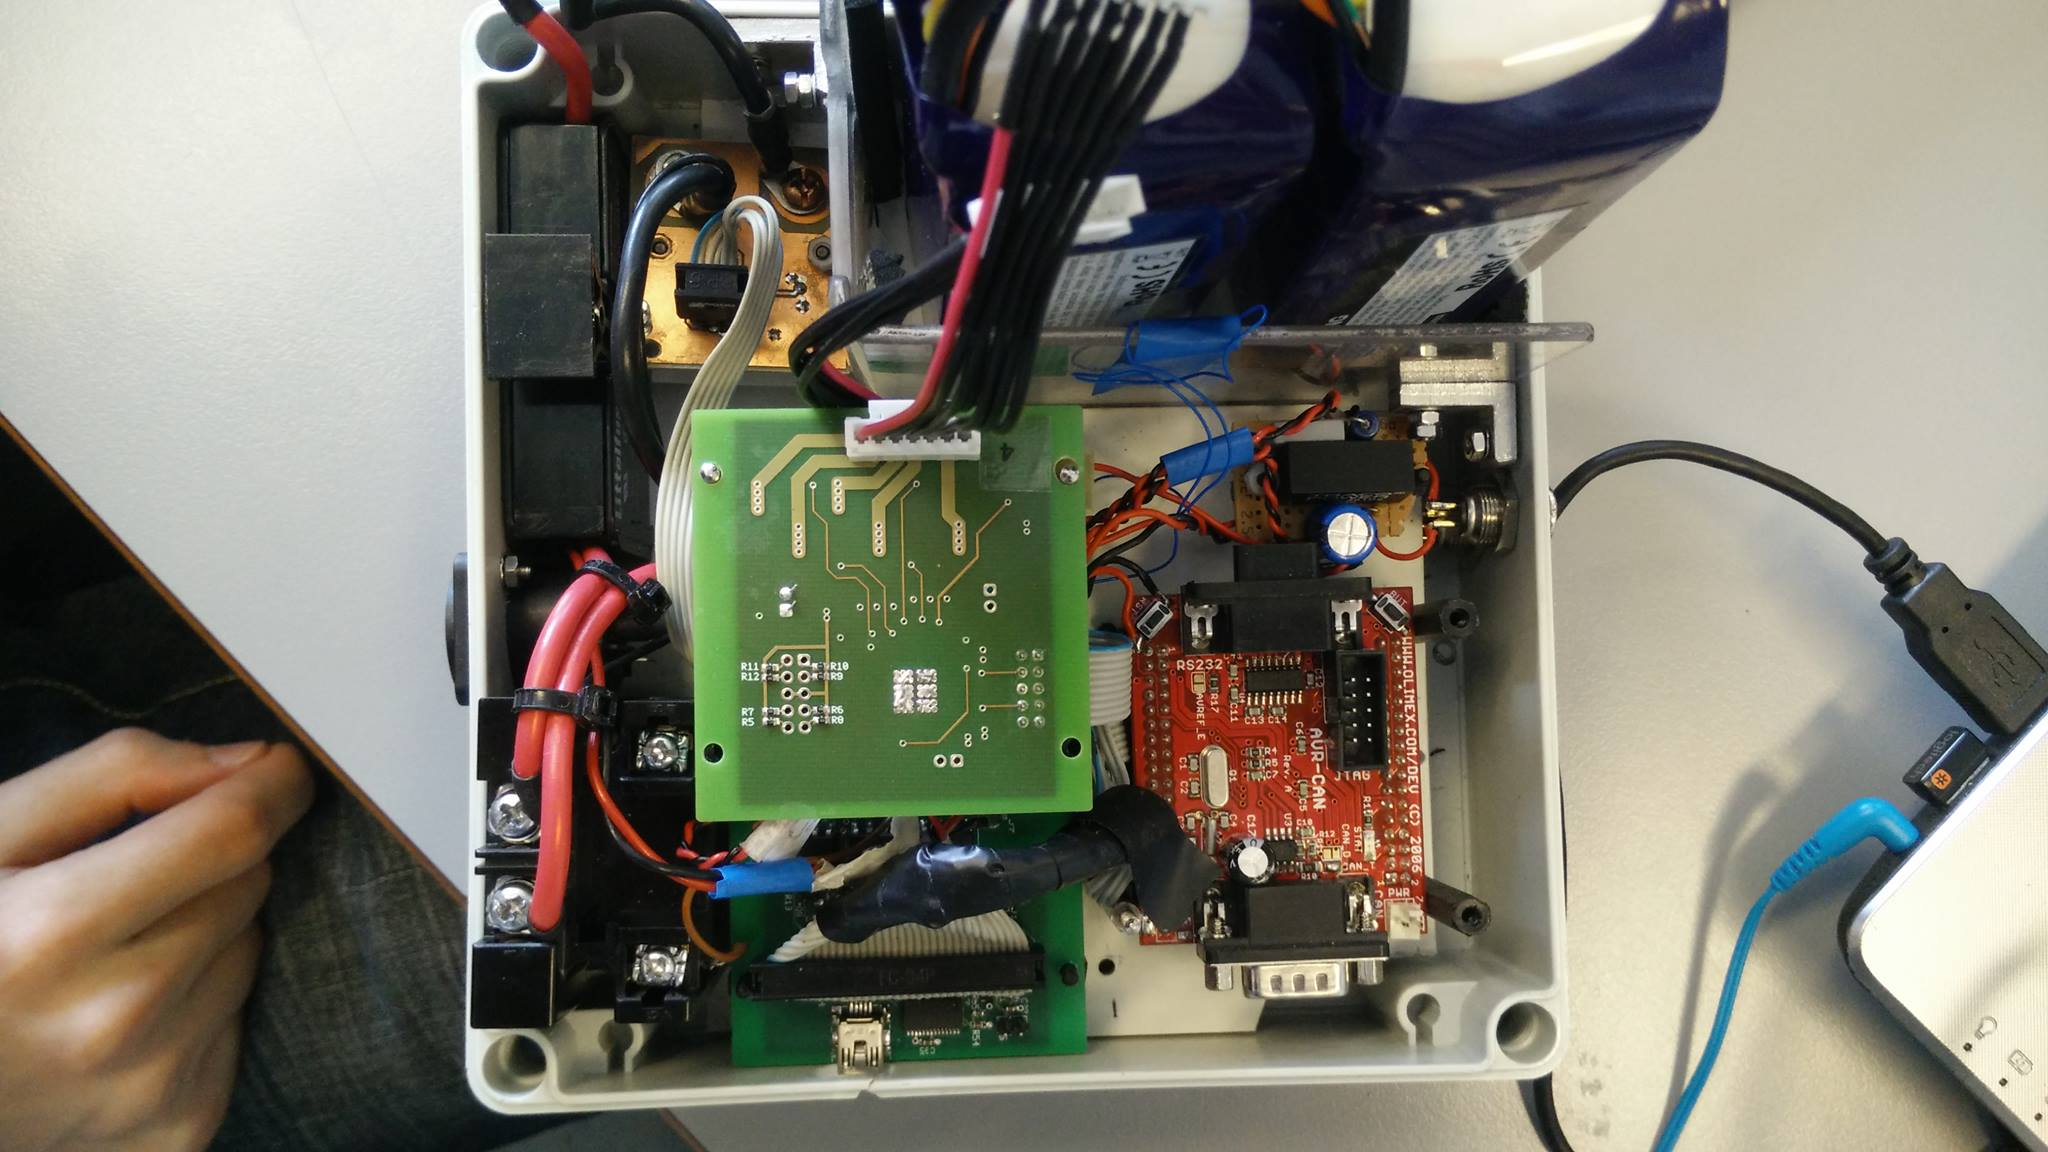
\includegraphics[width=0.7\linewidth]{SubPages/Images/SD_BMS}
	\caption{Battery manage system}
	\label{fig:SD_BMS}
\end{figure}

\section{Rolling Road}
The Controller-box containing the PCB and the PSoC can be seen in figure \vref{fig:SD_RR}. Around the edge of the box all external connections can be seen using banana-plugs, 12v-jack and USB. 

\begin{figure}[H]
	\centering
	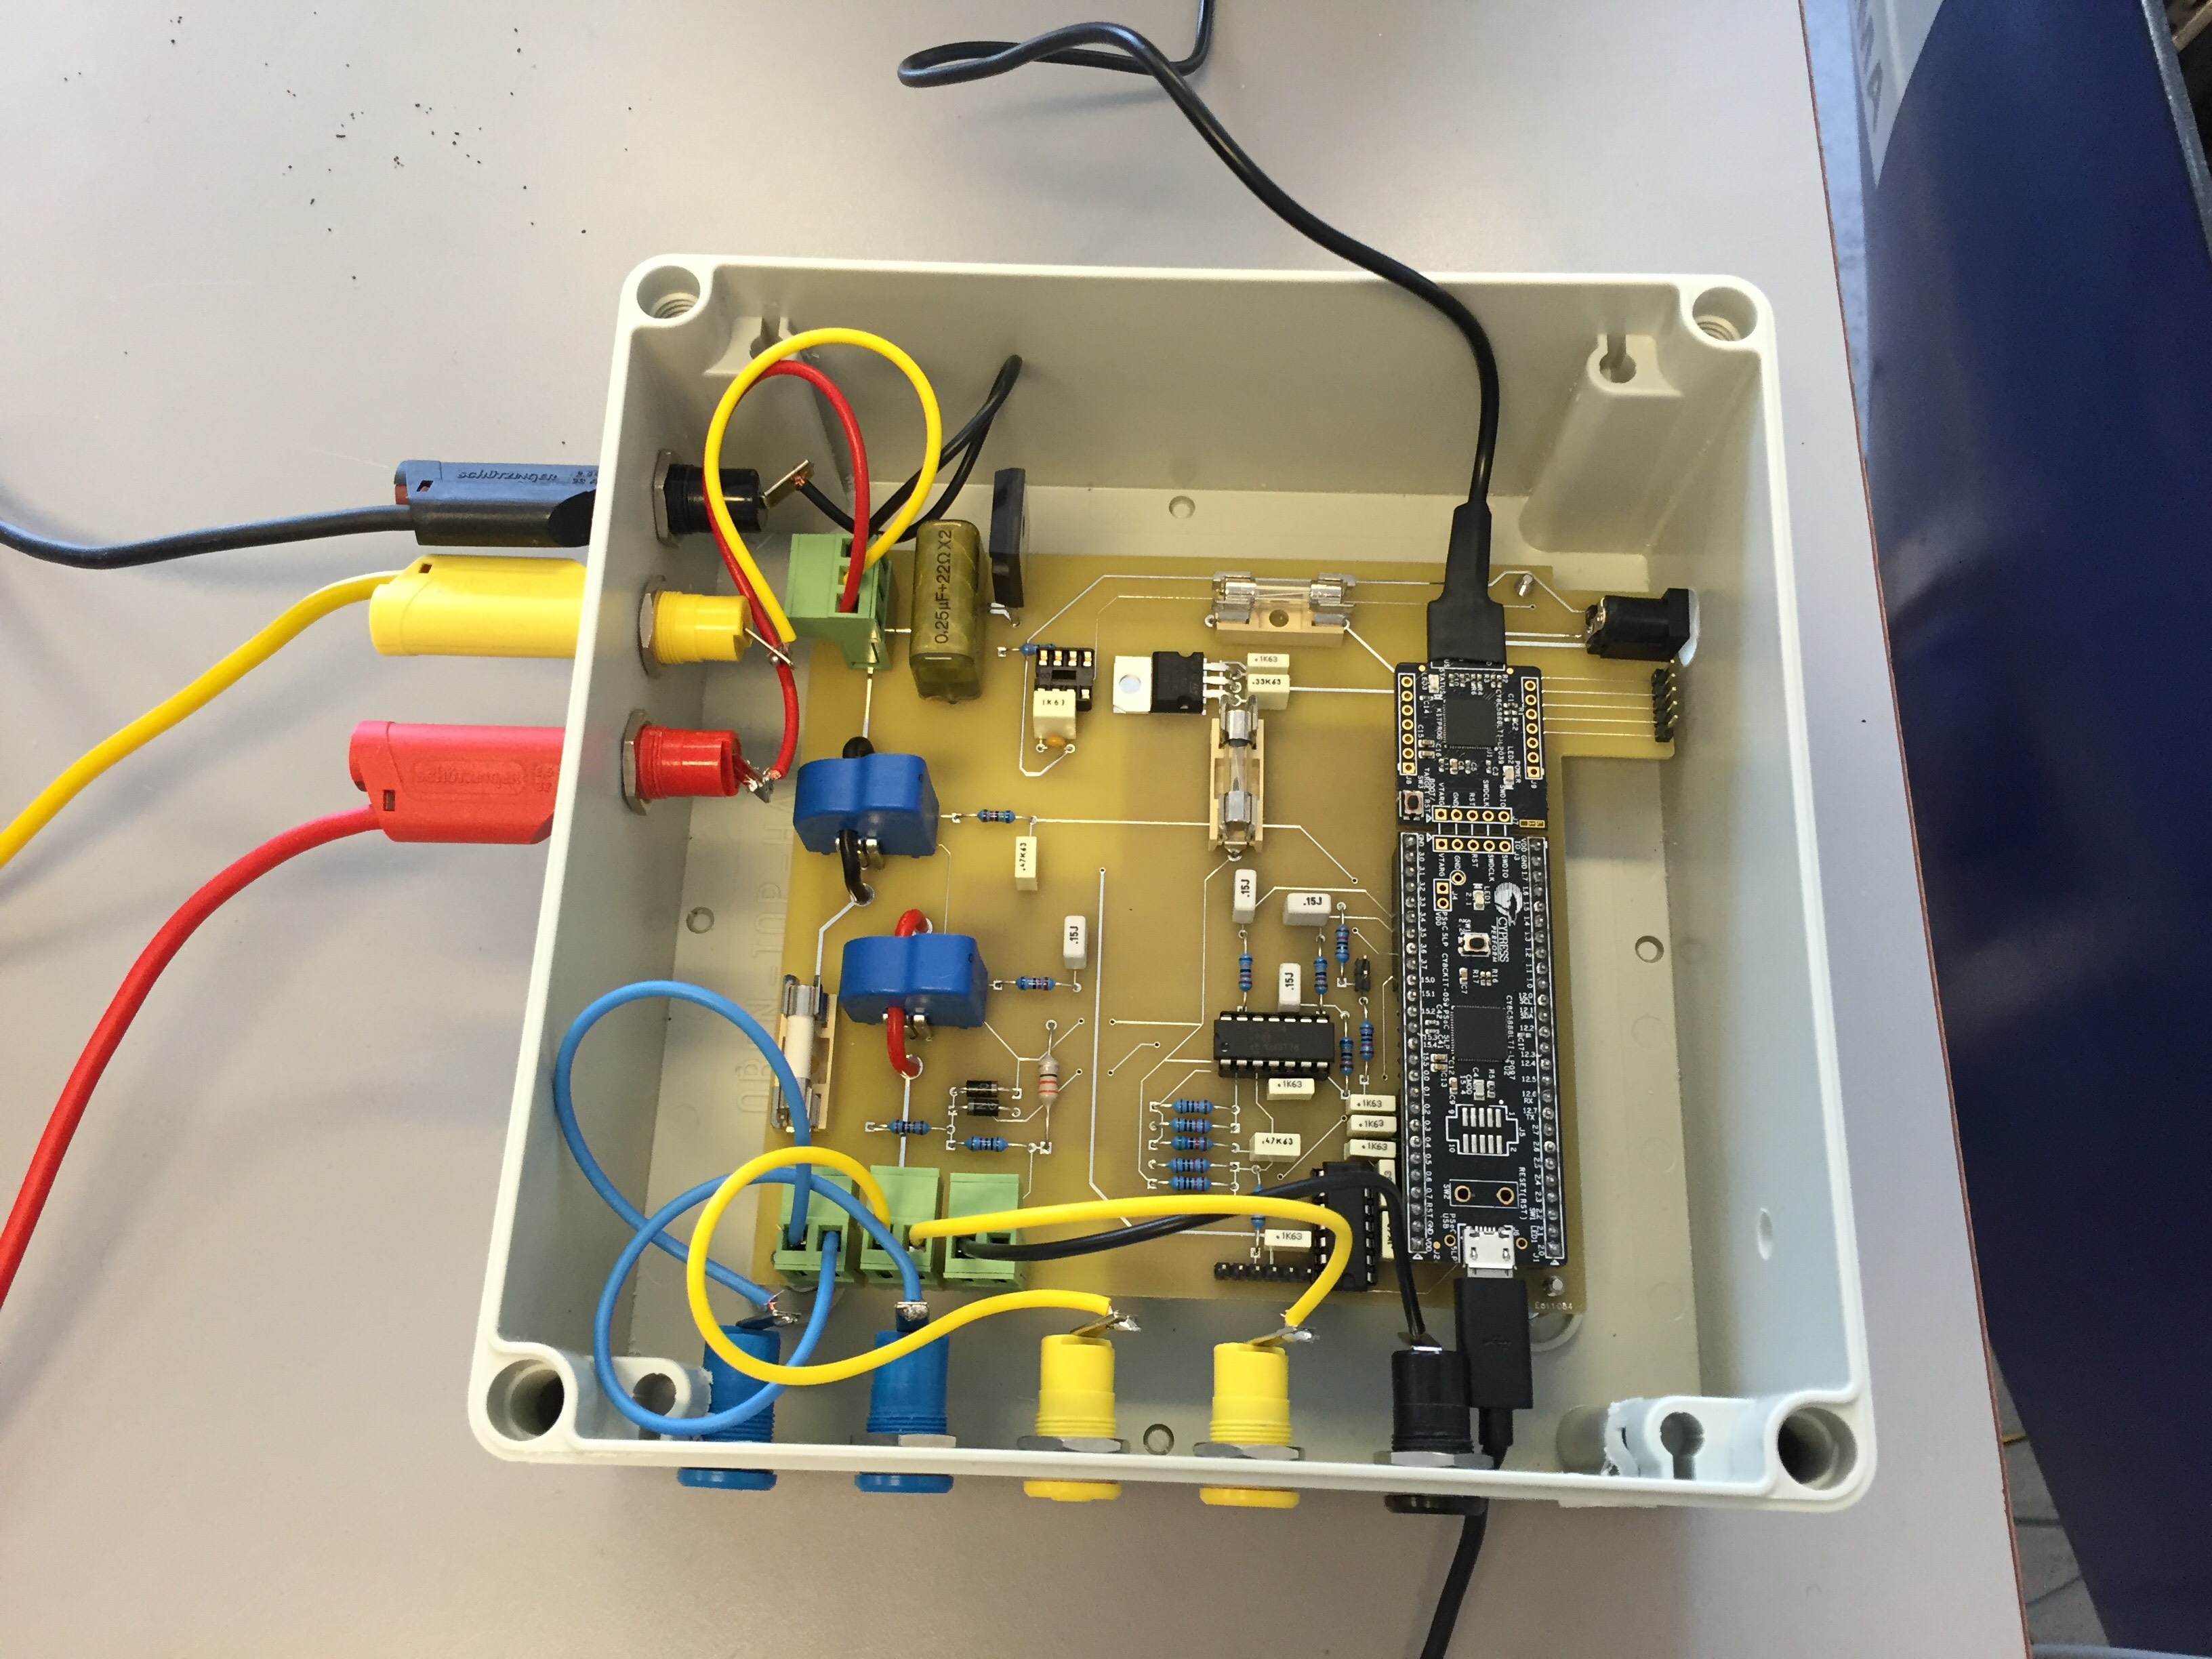
\includegraphics[width=0.7\linewidth]{SubPages/Images/SD_RR}
	\caption{Rolling Road Controller}
	\label{fig:SD_RR}
\end{figure}


The Physical stand containing the generator(right) and torque sensor(center) can be seen in figure \vref{fig:SS_RR_Roal}.

\begin{figure}[H]
	\centering
	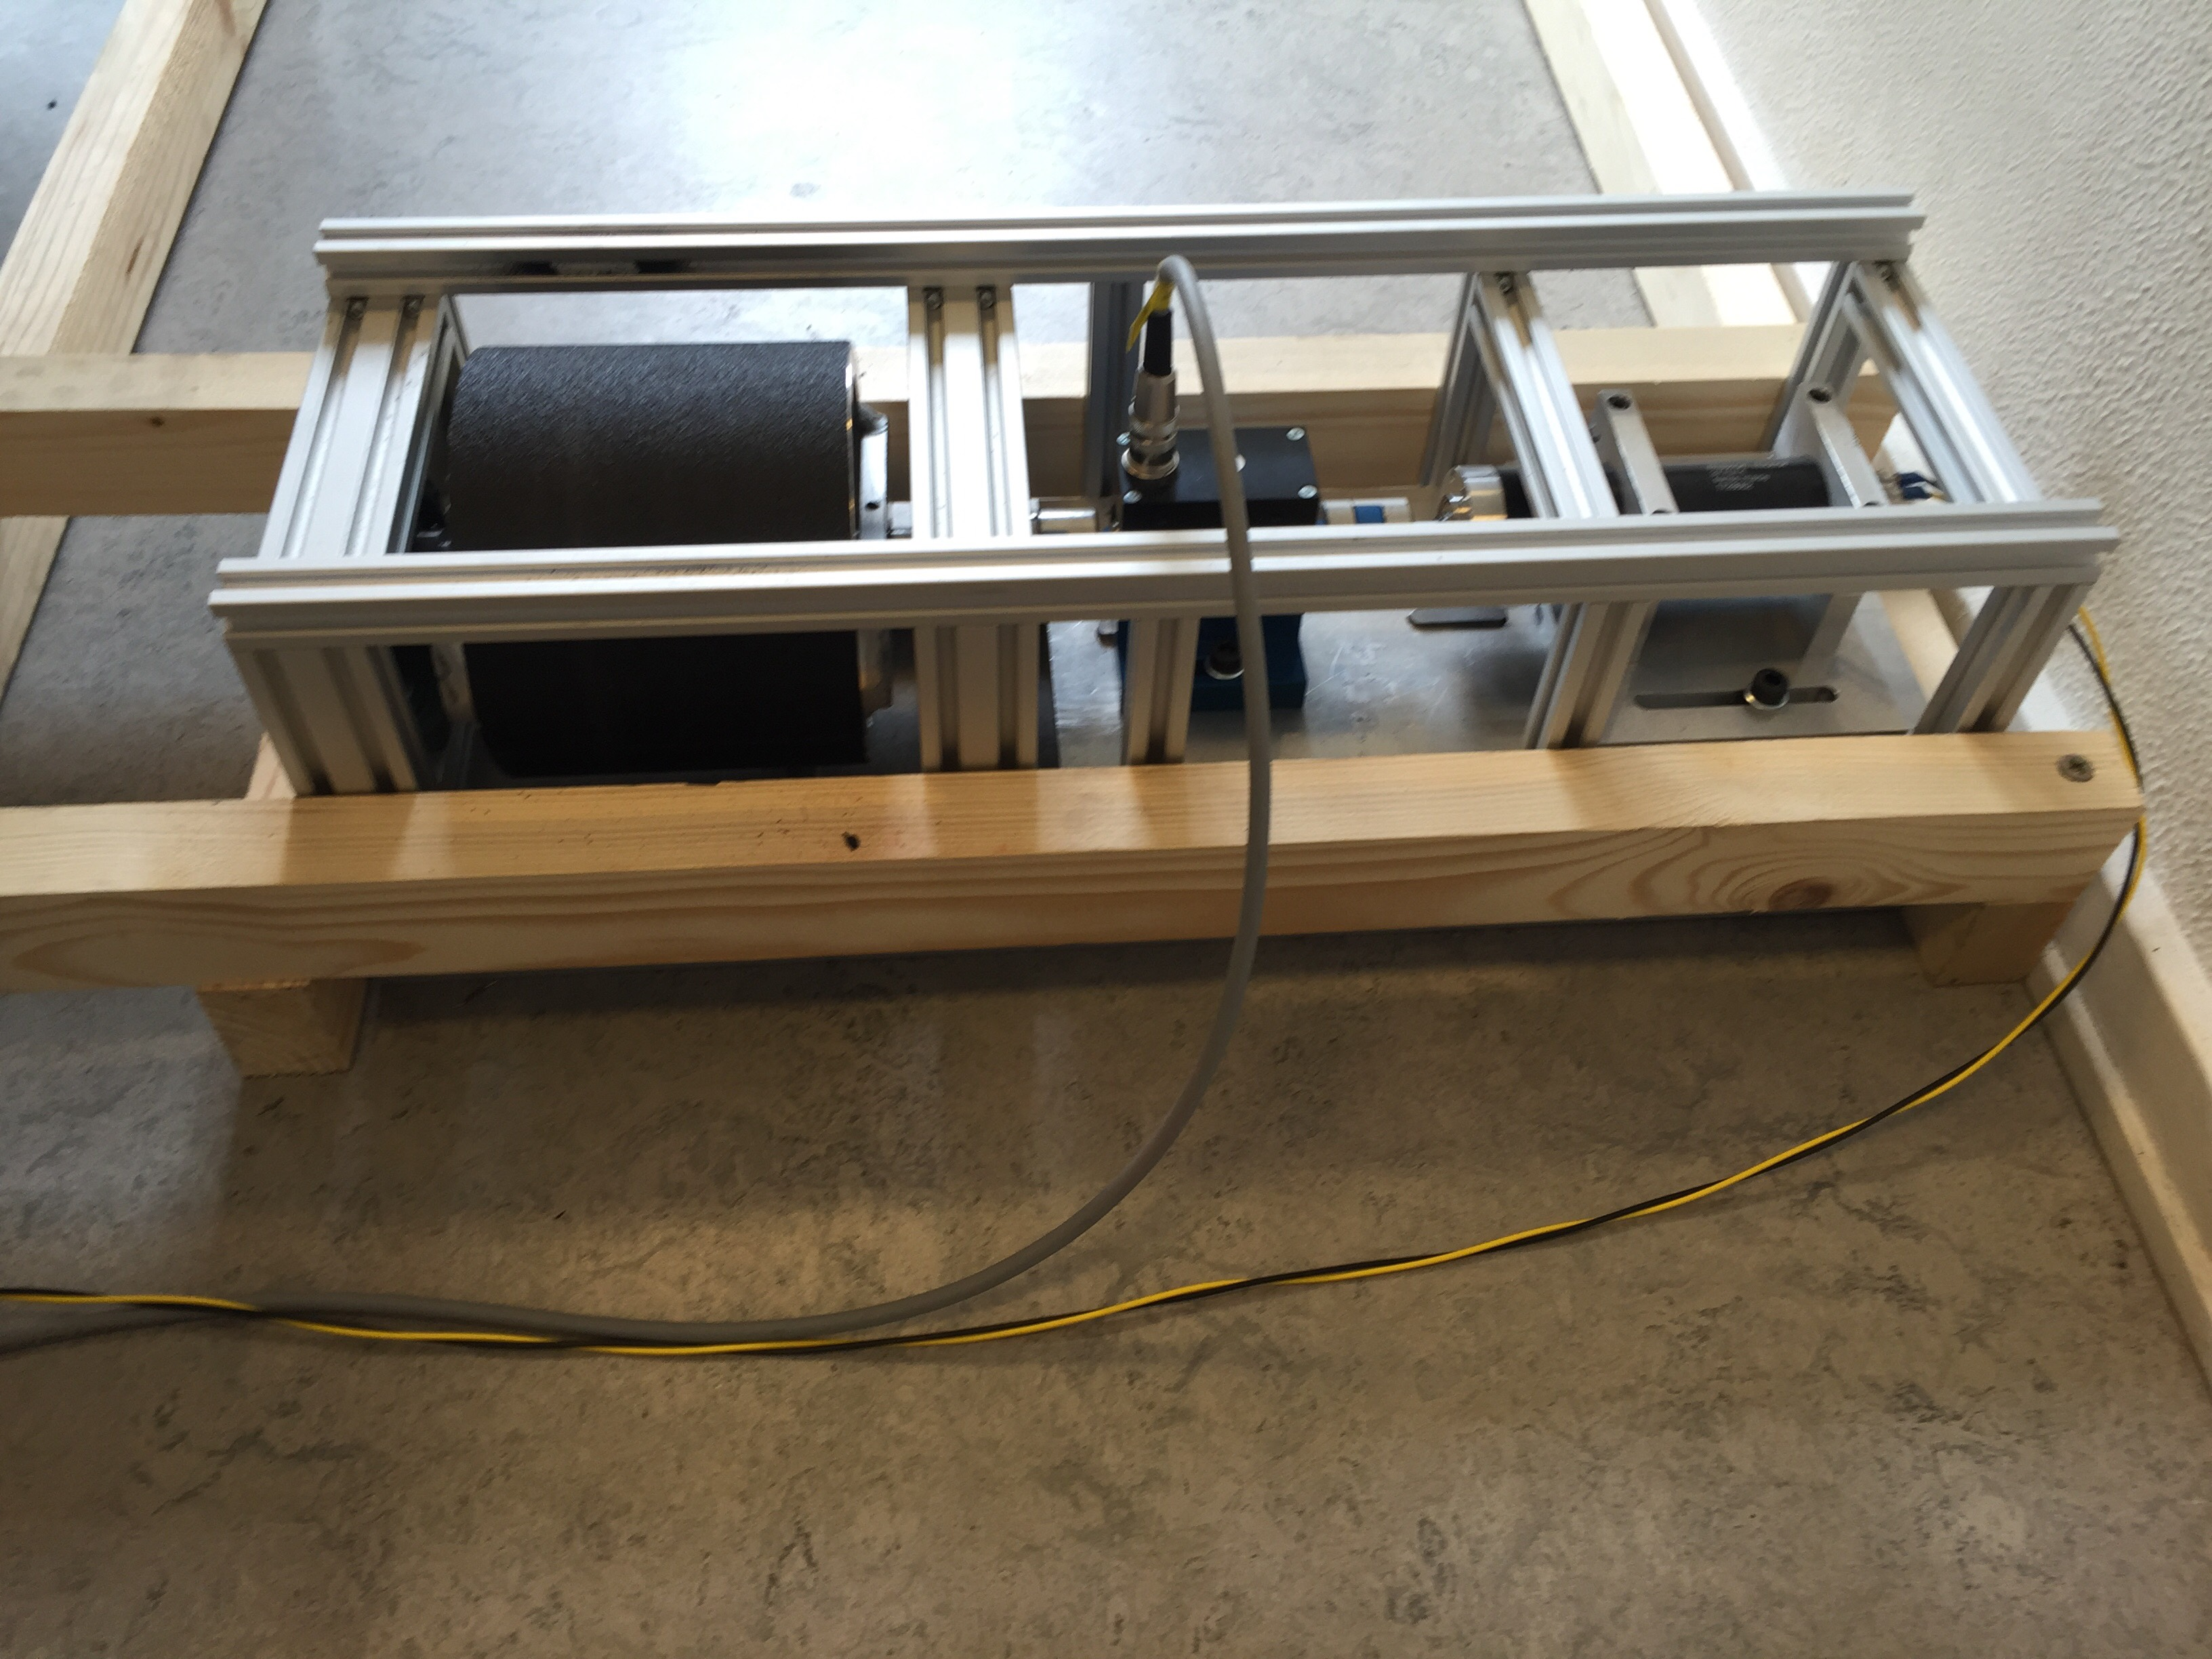
\includegraphics[width=0.7\linewidth]{SubPages/Images/SS_RR_Roal}
	\caption{Rolling Road}
	\label{fig:SS_RR_Roal}
\end{figure}

The Load-plate containing the super capacitor and the two power resistors:

\begin{figure}[H]
	\centering
	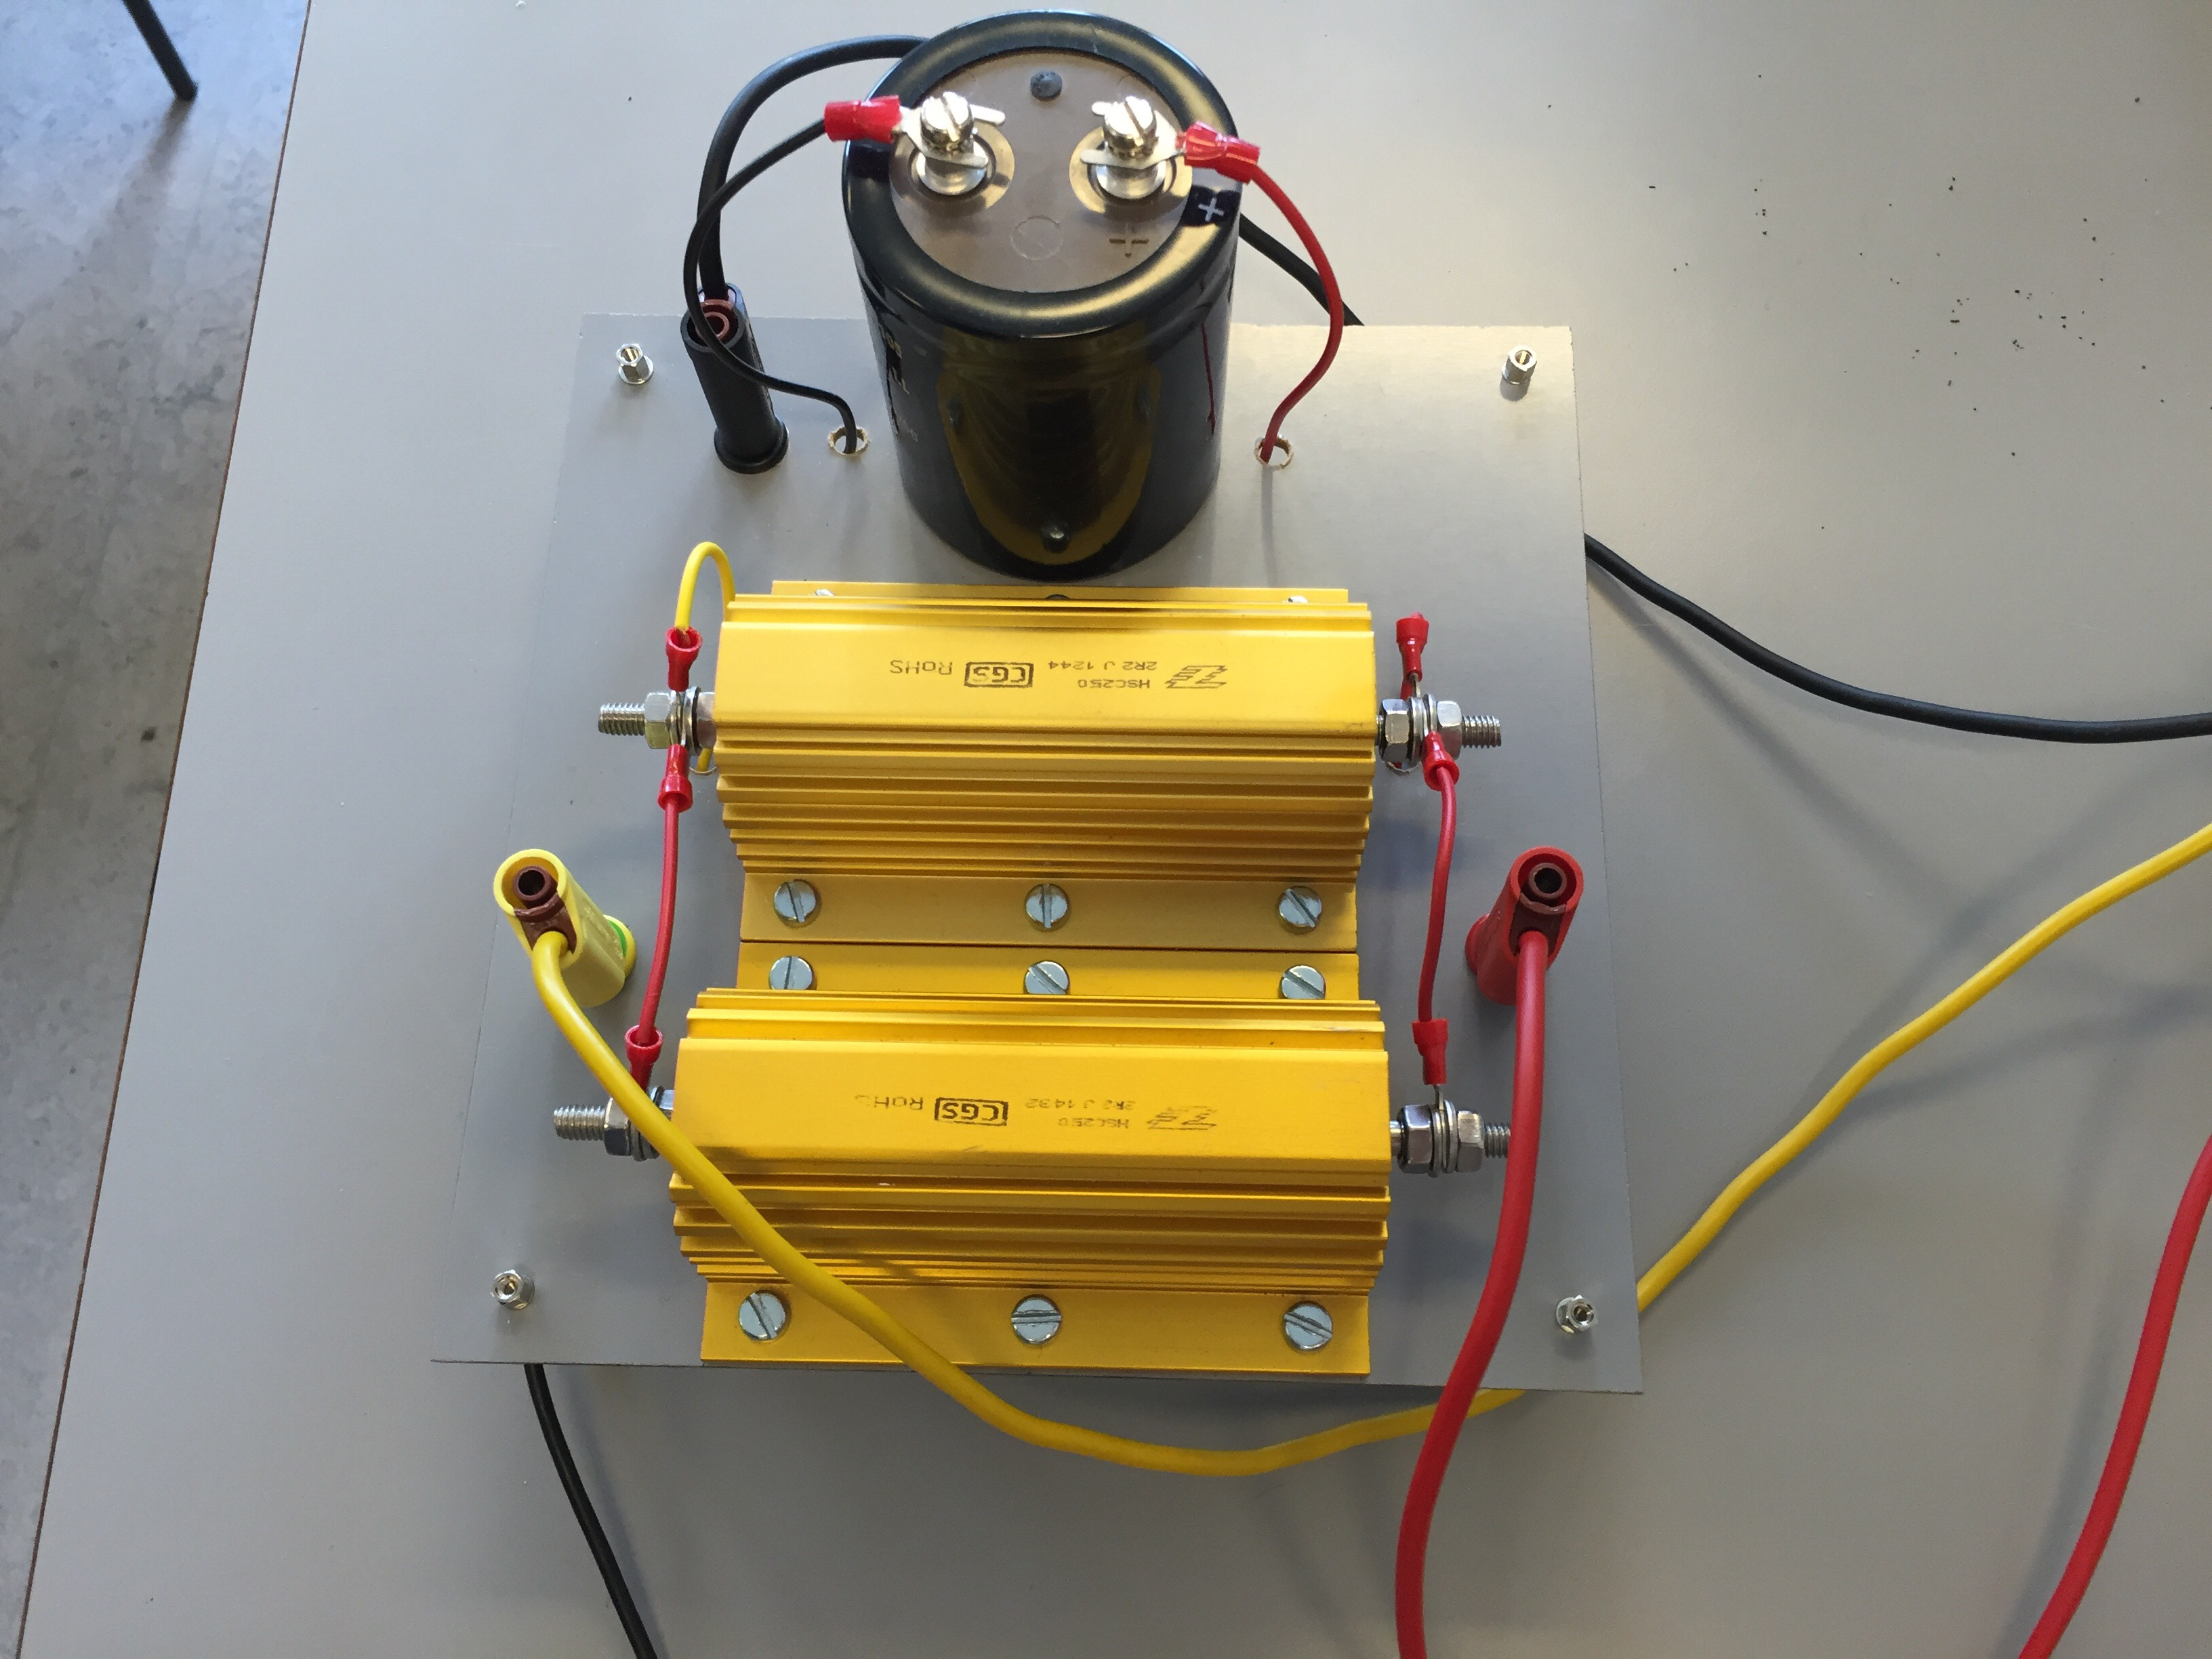
\includegraphics[width=0.7\linewidth]{SubPages/Images/SD_RR_Load}
	\caption{Load-plate}
	\label{fig:SD_RR_Load}
\end{figure}


\section{Rolling Road GUI}

The rolling road live-data display, where some simulated data has been collected and displayed to the used. To the left all the control would be available if connected to the Rolling Road, and to the right the latest readings from the Rolling Road can be seen.

\begin{figure}[H]
	\centering
	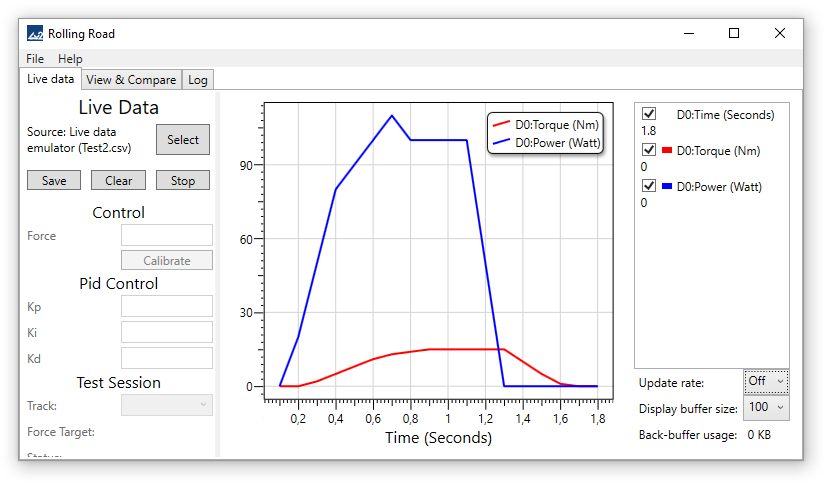
\includegraphics[width=0.9\linewidth]{SubPages/Images/SD_GUI}
	\caption{Rolling Road GUI}
	\label{fig:SD_GUI}
\end{figure}
